\documentclass{article}
\usepackage{calc}
\usepackage{graphicx}
\usepackage{float}
\usepackage{eso-pic}

\usepackage{array}    % For better column alignment
\usepackage{longtable} % For tables that span multiple pages
\usepackage{setspace}   % For adjusting line spacing
\usepackage{booktabs}   % For better looking tables (optional)
\usepackage{makecell}   % For custom cell formatting, especially for headings
\usepackage{hyperref}


\newlength{\PageFrameTopMargin}
\newlength{\PageFrameBottomMargin}
\newlength{\PageFrameLeftMargin}
\newlength{\PageFrameRightMargin}

\setlength{\PageFrameTopMargin}{0.8cm}
\setlength{\PageFrameBottomMargin}{0.8cm}
\setlength{\PageFrameLeftMargin}{0.8cm}
\setlength{\PageFrameRightMargin}{0.8cm}

% Increase padding inside cells
\renewcommand\arraystretch{2} % Increase row height
\setlength{\tabcolsep}{12pt}    % Increase horizontal padding (space between text and cell border)

\makeatletter

\newlength{\Page@FrameHeight}
\newlength{\Page@FrameWidth}

\AddToShipoutPicture{
  \thinlines
  \setlength{\Page@FrameHeight}{\paperheight-\PageFrameTopMargin-\PageFrameBottomMargin}
  \setlength{\Page@FrameWidth}{\paperwidth-\PageFrameLeftMargin-\PageFrameRightMargin}
  \put(\strip@pt\PageFrameLeftMargin,\strip@pt\PageFrameTopMargin){
    \framebox(\strip@pt\Page@FrameWidth, \strip@pt\Page@FrameHeight){}}}

\makeatother

\begin{document}

\begin{center}
    \Huge \underline{Lab Notebook}
\end{center}
    \vspace{1em}

    \begin{center}
    {\Large
    \underline{Software Tools and Technology Lab}} 
    \end{center}

    \vspace{0.4em}
    
    \begin{center}
        {\Large \underline{SEBCA1191}}
    \end{center}




\begin{figure}[h]
    \centering
    \includegraphics[width=0.75\linewidth]{front.PNG}
    
    \end{figure}

\vspace{1cm}

\begin{center}
    
\setlength{\arrayrulewidth}{0.4mm}
\setlength{\tabcolsep}{20pt}
\renewcommand{\arraystretch}{2}
\begin{tabular}{ |c|c|c| }
\hline
\multicolumn{3}{|c|}{\Large \textbf{\textit{Group 24}}} \\
\hline
NAME & ROLL NO.& DEPARTMENT \\
\hline
Snehal Das [Leader] & 30001223015 & BCA \\
Nupur Sinha & 30001223002 & BCA \\
Nikita Debnath & 30001223023 & BCA \\
Swastik Das & 30001223075 & BCA \\
Sunit Modak & 30084323005 & BSc in Data Science \\

\hline
\end{tabular}
\end{center}

\newpage

\begin{center}
    \Huge{\textit{\textbf{Index Page}}}

\vspace{1.1cm}
\end{center}


% Define the table with width 80% of textwidth
\begin{center}
    
\large \begin{longtable}{|p{0.08\textwidth}|p{0.13\textwidth}|p{0.45\textwidth}|p{0.145\textwidth}|}
    \hline
    \textbf{\Large S.No.} & \textbf{\Large Subject} & \textbf{\Large Description} & \textbf{\Large Pages} \\
    \hline
    \endfirsthead
    \hline
    \textbf{\Large S.No.} & \textbf{\Large Subject} & \textbf{\Large Description} & \textbf{\Large Pages} \\
    \hline
    \endhead
    \hline
    1 & Calculator & Download GitHub desktop in your system, create a local repository. Build a C programme of calculator in the local repository, commit and publish it as a public repository. & 3-4 \\
    \hline
    2 & Sections and Subsections & How to create sections and subsection in LaTeX in a proper manner. & 5-6 \\
    \hline
    3 & CV using LaTeX & Your task is to create your CV using LaTeX documen & 7-8 \\
    \hline
    4 & Mathematical Document & Your task is to create your LaTeX document. 
    The document should be formatted to look exactly like an attachment. & 9-10 \\
    \hline
    5 & Git Branching and Merging & A hands-on task to understand and implement Branching, Merging, conflict resolution in Git. & 11-12 \\
    \hline
    
    
\end{longtable}
\end{center}
\newpage

\begin{center}
    \Huge I. \underline{Calculator Repository}
    \end{center}
    \vspace{1em}

    \begin{center}
        \Large GitHub Desktop
    \end{center}

    \vspace{0.4em}
    
    \begin{center}
        \large 09/08/2024
    \end{center}


\section{\underline{Description:}}
The task was divided into two parts: \vspace{0.2cm}\newline

1. Download GitHub desktop in your system (https://desktop.github.com/download/) and go through the tutorial for private repository publish. \vspace{0.2cm}
\newline

2. Create a local repository. Build a C programme of calculator in the local repository, commit and publish it as a public repository. \vspace{0.2cm}
\newline

\section{\underline{Steps:}}
The task was achieved by following the below mentioned steps:-
\newline

1. Download the GitHub Desktop Application through the given link. Then basic account setup. \vspace{0.5cm}

2. Using the OPEN IN SUBMILE TEXT (whichever text editor you have) option, update README file. Come back to app, and commit the change, using meaningful message. \vspace{0.5cm}

3. In your Desktop Application, go to file --> New Repository --> Give Name, Description, and specify local path. Check or uncheck README file and --> Create Repository \vspace{0.5cm}

4. In text editor, create a C file called basicCalculator, and write your code, save. Using similar steps, commit the change. \vspace{0.5cm}

5. Now Publish Repository, to push the repo into remote Git server. \vspace{0.5cm}

\newpage
\subsection{\underline{Code Snippet:}}

\begin{figure}[h!]
    \centering
    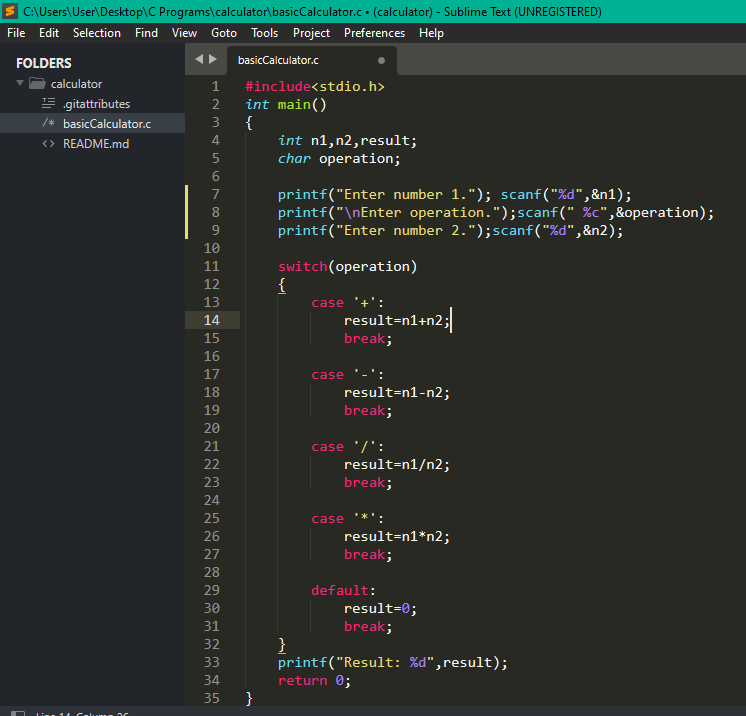
\includegraphics[width=0.7\textwidth]{calculator1.PNG}
    \caption{Source Code}
\end{figure}

\centering

\large This is a simple Calculator program in C, which takes in 3 inputs from the user- the two operands, and the operator. The program makes use of the SWITCH CASE statement to implement conditions, calculating and displaying the result accordingly.

\vspace{1.3cm}

\begin{figure}[h!]
    \centering
    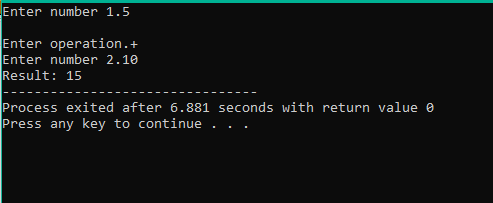
\includegraphics[width=0.7\textwidth]{calculator2.PNG}
    \caption{Output}
\end{figure}

\newpage

\begin{center}
    \LARGE{\textbf{2. \underline{Lab Assignment by Nupur Sinha}}}
\end{center}
\vspace{0.2cm}
 \begin{center}
     \section*{\underline{How to create Matrix in LaTeX}}
\end{center}
\LARGE{To create a matrix in LaTeX, we use the \texttt{\textbf{amsmath}} package, which provides various environments for displaying matrices. Here’s a basic guide on how to create a matrix and the different options available:}
\vspace{0.1cm}
\begin{center}
\begin{itemize}
    \item{\underline{\textbf{Include the \texttt{amsmath} Package}}}
\end{itemize} 
\end{center}
First, ensure you have the \texttt{amsmath} package included in your LaTeX document preamble. Add the following line:
\begin{verbatim}
\usepackage{amsmath}
\end{verbatim}
\begin{center}
    \begin{itemize}
        \item {\textbf{\underline{Matrix Environments}}}
    \end{itemize}
\end{center}
\LARGE{
There are several environments for creating matrices, depending on how you want them formatted. Here are the most common ones:}

\begin{itemize}
  \item \texttt{matrix}: A basic matrix without brackets.
  \item \texttt{bmatrix}: A matrix with square brackets.
  \item \texttt{pmatrix}: A matrix with parentheses.
  \item \texttt{vmatrix}: A matrix with vertical bars.
  \item \texttt{Vmatrix}: A matrix with double vertical bars.
\end{itemize}
\begin{center}
        \item {\textbf{\underline{\LARGE{Syntax}}}}
\end{center}

\LARGE{The syntax for creating a matrix is similar across different environments. Use the \texttt{\textbackslash begin\{environment\}} and \texttt{\textbackslash end\{environment\}} commands to enclose the matrix content. Separate the elements in each row with \texttt{\&} and 

end each row with \texttt{\\}.

Here’s an example of a 2x2 matrix in each environment:}
\begin{verbatim}
[ 
$ \begin{matrix}
    1 & 0 \\
    0 & 1 
\end{matrix}
$ ]

\begin{bmatrix}   [
 $   \begin{matrix}
    1 & 0\\
    0 & 1
    \end{matrix}
 $   ]

a_{11} & a_{12} \\
a_{21} & a_{22}
\end{bmatrix}

\begin{pmatrix}
a_{11} & a_{12} \\
a_{21} & a_{22}
\end{pmatrix}

\begin{vmatrix}
a_{11} & a_{12} \\
a_{21} & a_{22}
\end{vmatrix}

\begin{Vmatrix}
a_{11} & a_{12} \\
a_{21} & a_{22}
\end{Vmatrix}
\end{verbatim}

\begin{center}
\section*{\textbf{\underline{\LARGE{Explanation}}}}
\end{center}
\begin{itemize}
  \item \texttt{\textbackslash begin\{matrix\} ... \textbackslash end\{matrix\}}: Creates a matrix with no surrounding brackets.
  \item \texttt{\textbackslash begin\{bmatrix\} ... \textbackslash end\{bmatrix\}}: Surrounds the matrix with square brackets.
  \item \texttt{\textbackslash begin\{pmatrix\} ... \textbackslash end\{pmatrix\}}: Surrounds the matrix with parentheses.
  \item \texttt{\textbackslash begin\{vmatrix\} ... \textbackslash end\{vmatrix\}}: Surrounds the matrix with single vertical bars, often used to denote determinants.
  \item \texttt{\textbackslash begin\{Vmatrix\} ... \textbackslash end\{Vmatrix\}}: Surrounds the matrix with double vertical bars, also used for determinants or norms.
\end{itemize}


\end{document}
